\documentclass[main]{subfiles}
\begin{document}

\chapter{Montaje}
\label{chap:montaje}

Al adquirir una plataforma comercial ya diseñada, no se dispone de espacio extra para instrumentarla. Se agregó una placa de sensores, una placa de desarrollo, una batería independiente para la electrónica, un GPS y un módulo Wi-Fi USB. Asimismo, para compatibilizar los diferentes voltajes que utilizaba cada placa, fue necesario hacer un circuito impreso que convirtiera los niveles lógicos de las señales.\\

A la hora de realizar el montaje de cada uno de los dispositivos mencionados, fue necesario realizar algunas consideraciones particulares. A continuación se presenta a grandes rasgos el trabajo de montaje realizado.

\section{BeagleBoard}

Se coloc\'o la \emph{BeagleBoard} junto con la batería de la electrónica (\emph{Beagle-Juice}) en la parte inferior del cuadricóptero. Considerando que la \emph{BeagleBoard} tiene una masa de $70g$ y la \emph{Beagle-Juice} alrededor de $125g$, la ubicación juega un rol fundamental en la posición del centro de masa del sistema global.\\

\begin{wrapfigure}{r}{0.55\textwidth}
%\begin{figure}[h!]
	\centering
	\vspace{-20pt}
		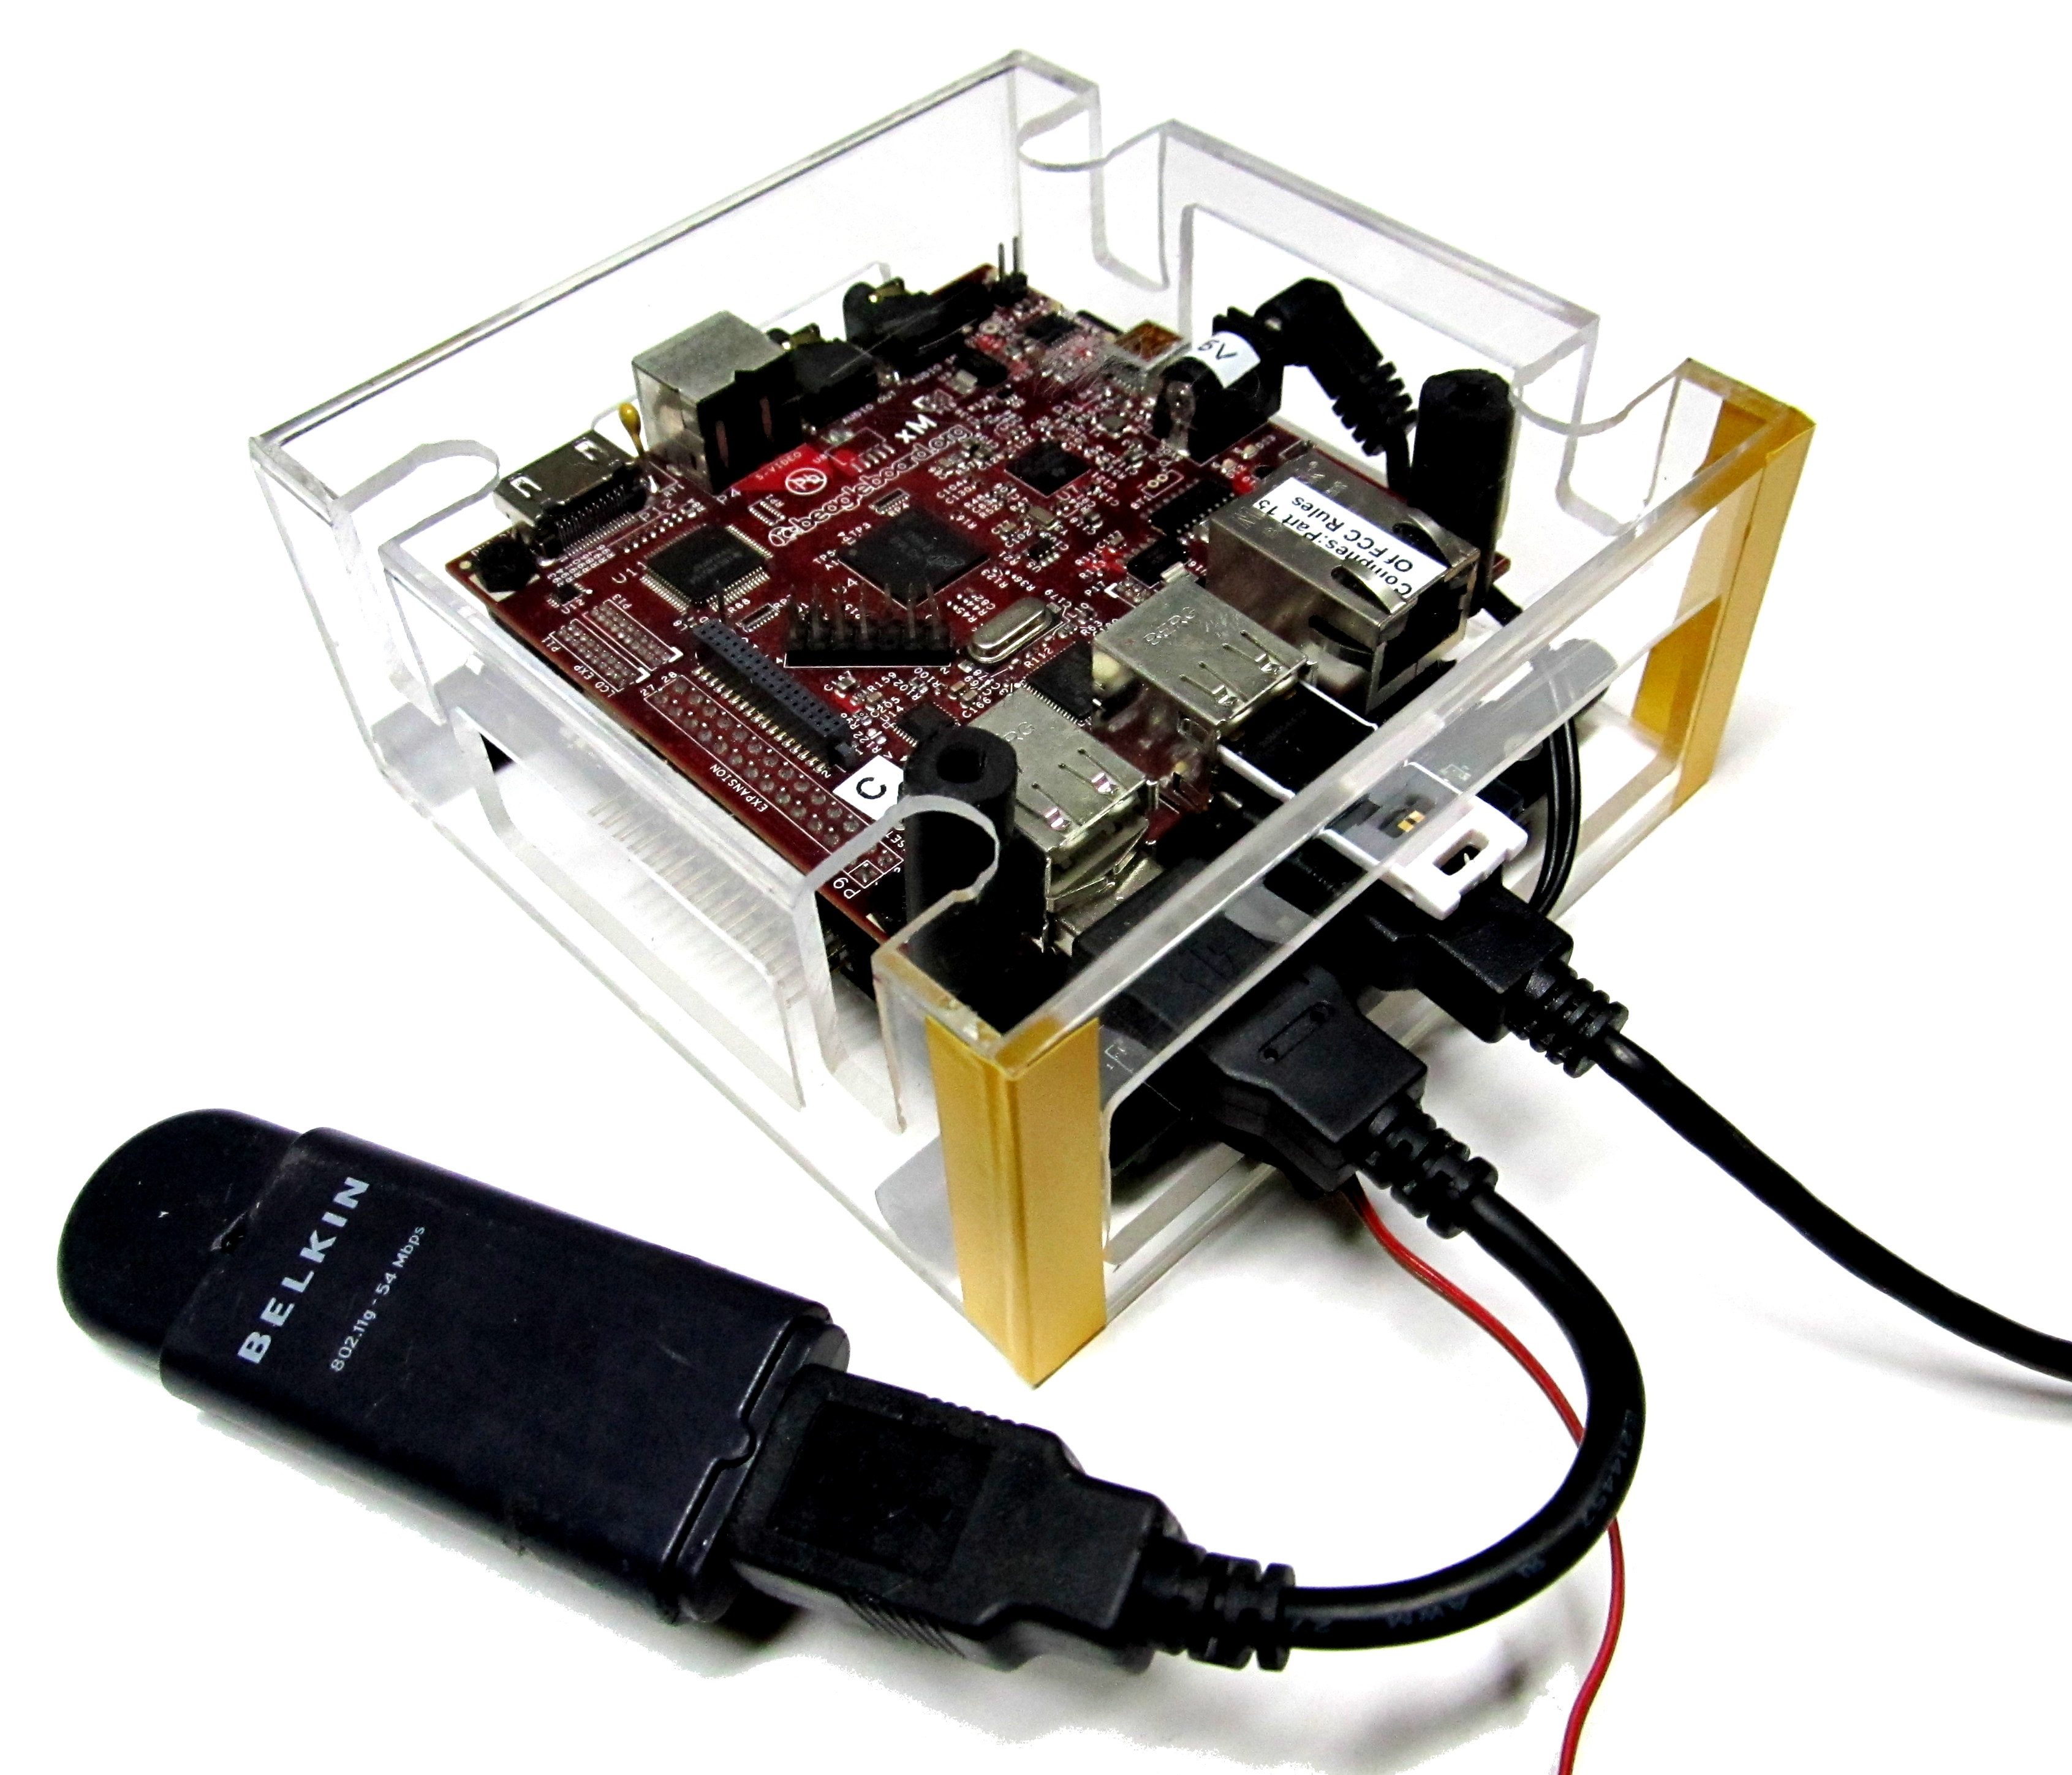
\includegraphics[width=0.5\textwidth]{./pics_montaje/beagle.jpg}
	\caption{Montaje del $BeagleBoard$}
	\vspace{-20pt}
	\label{fig:beagle}
%\end{figure}
\end{wrapfigure}

Se decidió ubicar las placas mencionadas en la parte inferior del cuadricóptero, implicando que el centro de masa del sistema se ubique algunos centímetros más abajo del centro geométrico, lo cual ayuda al sistema a lograr la estabilidad.\\

La \emph{BeagleBoard} se monta sobre la \emph{Beagle-Juice} mediante 4 tornillos de plástico con un tarugo (también de plástico) entre medio de ambas placas, de manera de mantenerlas solidarias y aisladas. En la imagen \ref{fig:beagle} se muestra la \emph{BeagleBoard} con la batería en una caja de acrílico pensada para protegerlas ante eventuales golpes. En la misma figura se puede observar además el módulo \emph{Wi-Fi} que es ubicado lo más hacia el exterior posible, de modo de minimizar los obstáculos a la señal.

\section{IMU}

La ubicación y montaje de la placa de sensores juega un papel fundamental a la hora de obtener las medidas. Se deben tomar algunas consideraciones que juegan un rol fundamental para poder lograr el control del cuadricóptero.\\

\begin{wrapfigure}{l}{0.5\textwidth}
	\begin{center}
		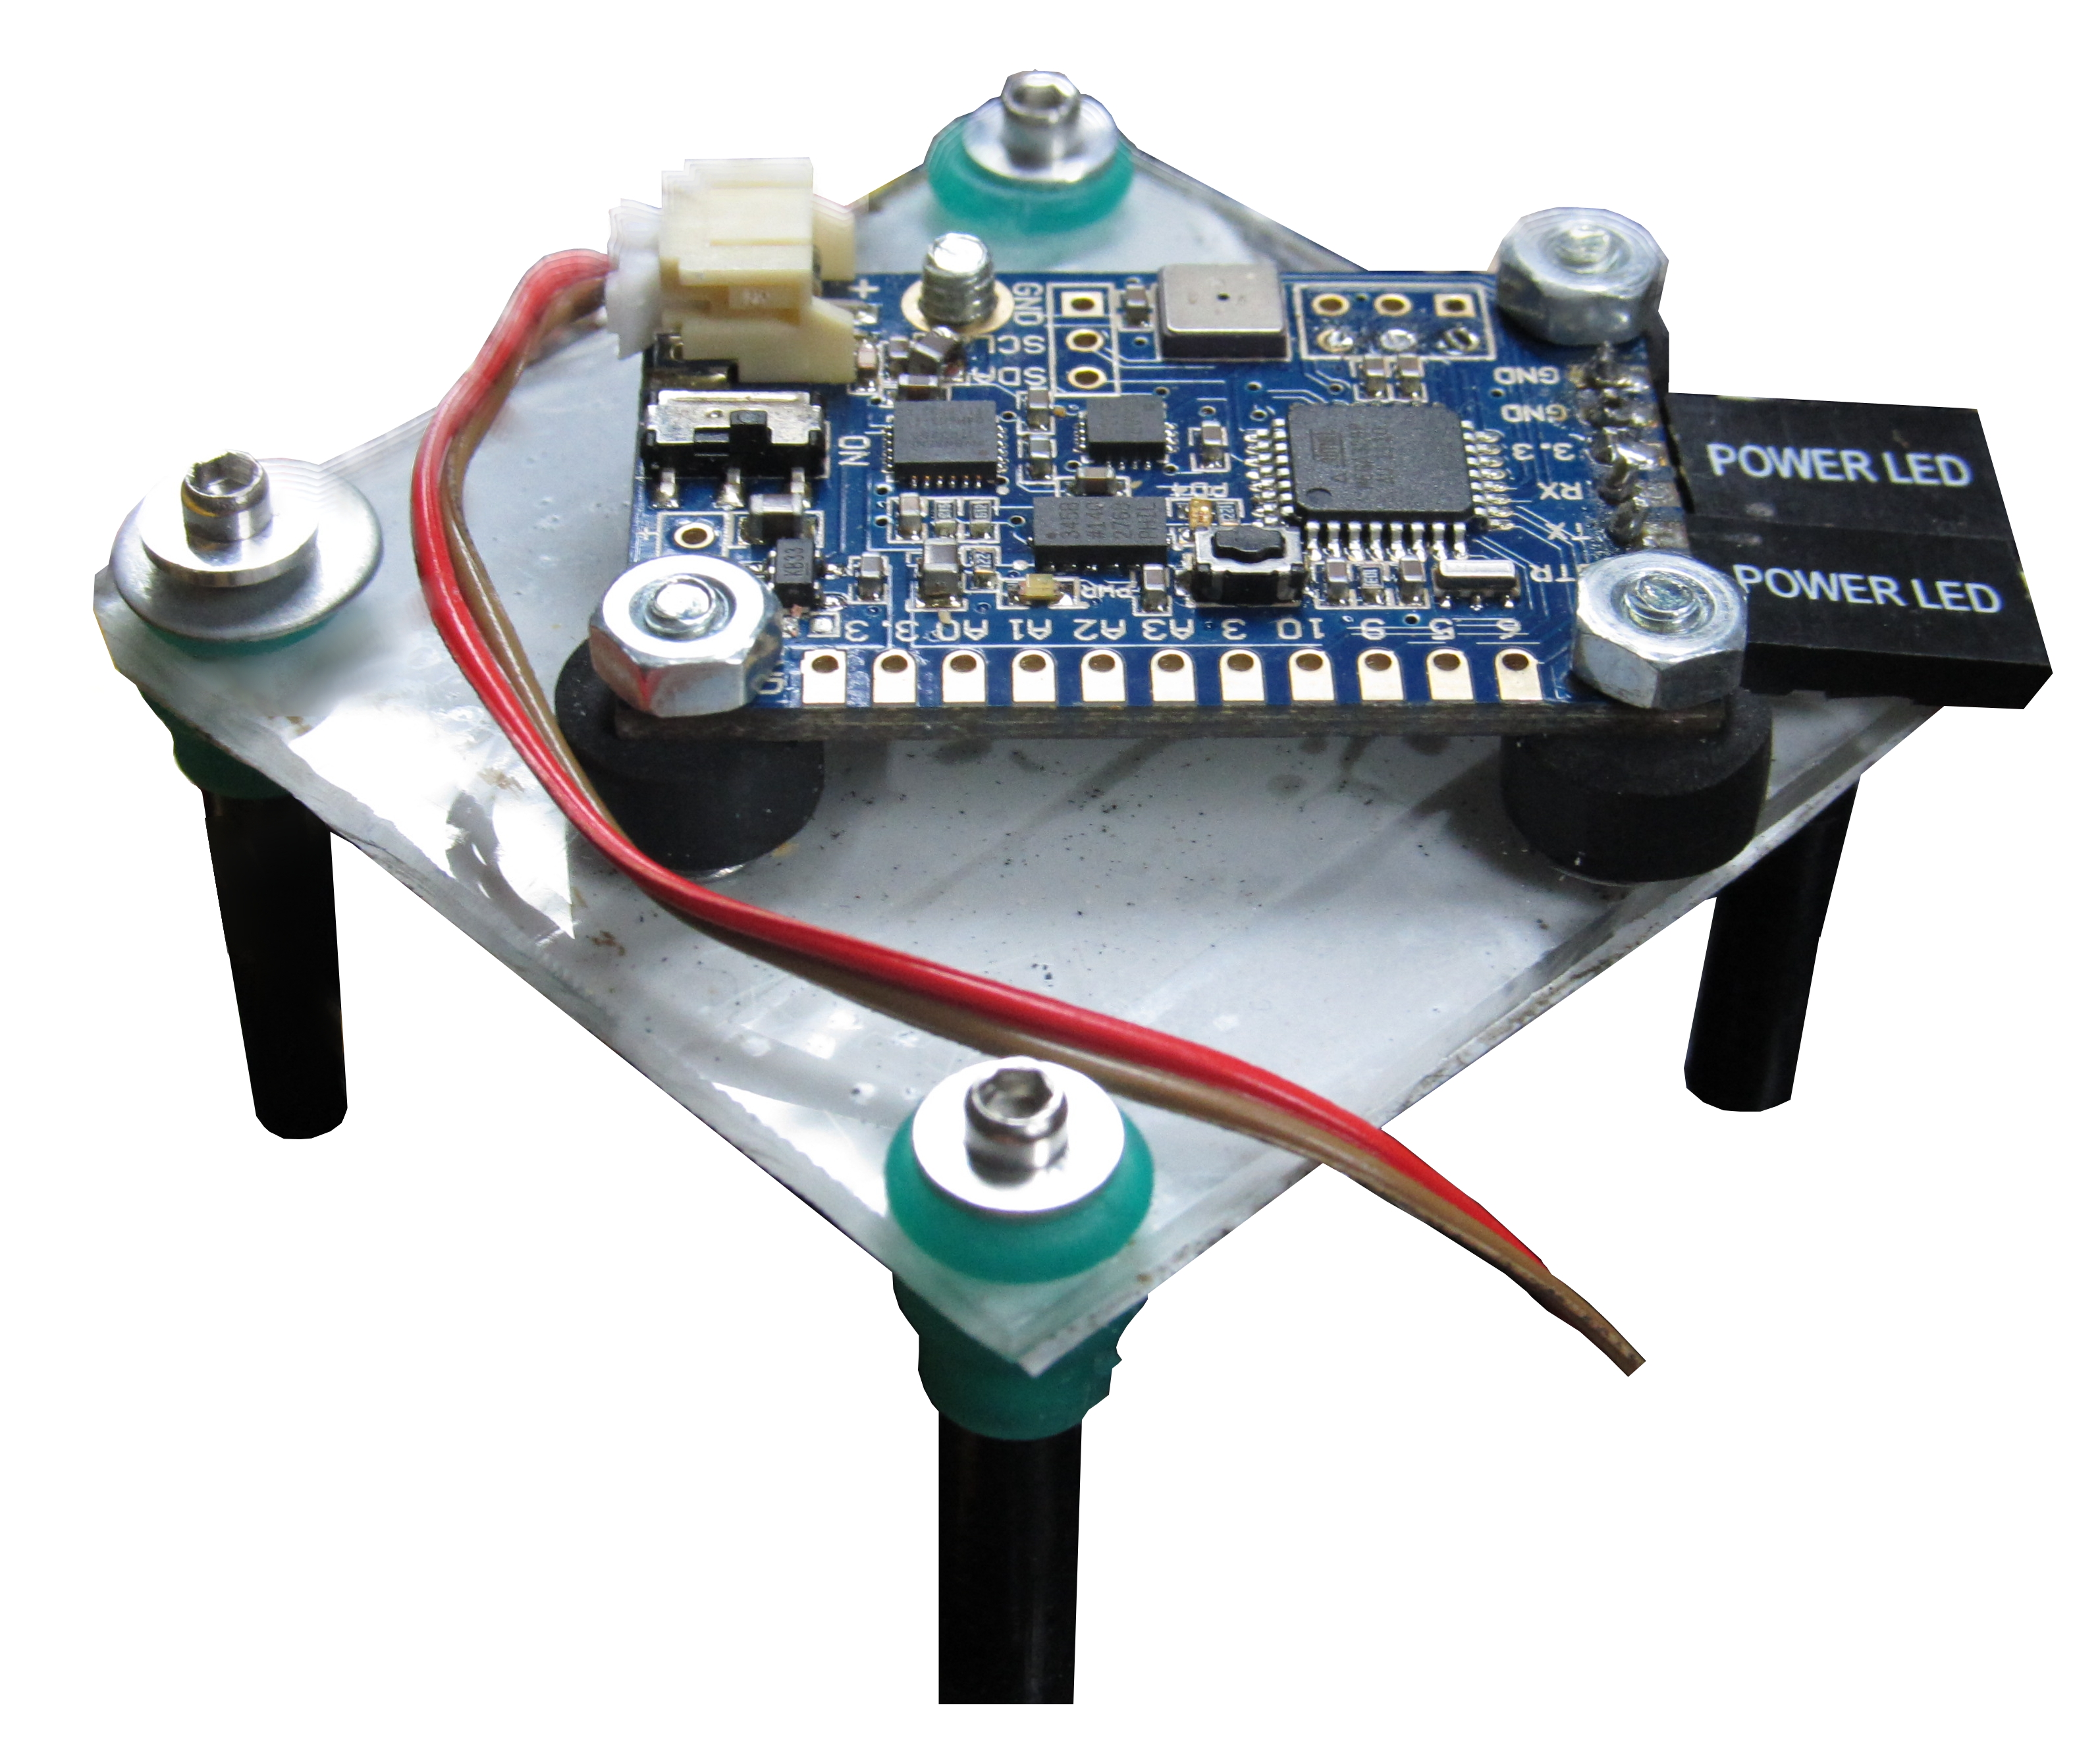
\includegraphics[width=0.45\textwidth]{./pics_montaje/imu.jpg}
	\end{center}
	\caption{Montaje de la IMU}
	\label{fig:imu}
\end{wrapfigure}

En primer lugar es importante que la placa se ubique en el centro del sistema. Más exactamente se deben ubicar a los acelerómetros de la placa lo más cerca del centro de masa posible, de modo de poder aproximar las aceleraciones medidas como las del centro de masa del cuadricóptero.\\

En la figura \ref{fig:imu} se muestra el montaje de la IMU, donde se utilizaron cuatro apoyos con los que contaba la plataforma, ubicados en el centro de la misma. La IMU se fija a una placa de acrílico que a su vez está fijada a dichos apoyos mediante amortiguadores de doble fuelle. Esto último es sumamente importante para disminuir el ruido de medida. Al encender los motores el ruido mecánico ocasionado provoca un aumento en el ruido de los sensores, llegando a tomar valores 10 veces mayores que con los motores apagados. Por esta razón resulta vital la amortiguación en el montaje de la placa. Los amortiguadores utilizados constan de 1 sola pieza que pasa por un agujero en la placa, logrando que la misma no tenga contacto directo ni con la carrocería ni con el tornillo, dejándola aislada de los elementos que vibran solidarios los motores.\\

\begin{wrapfigure}{r}{0.55\textwidth}
	\begin{center}
		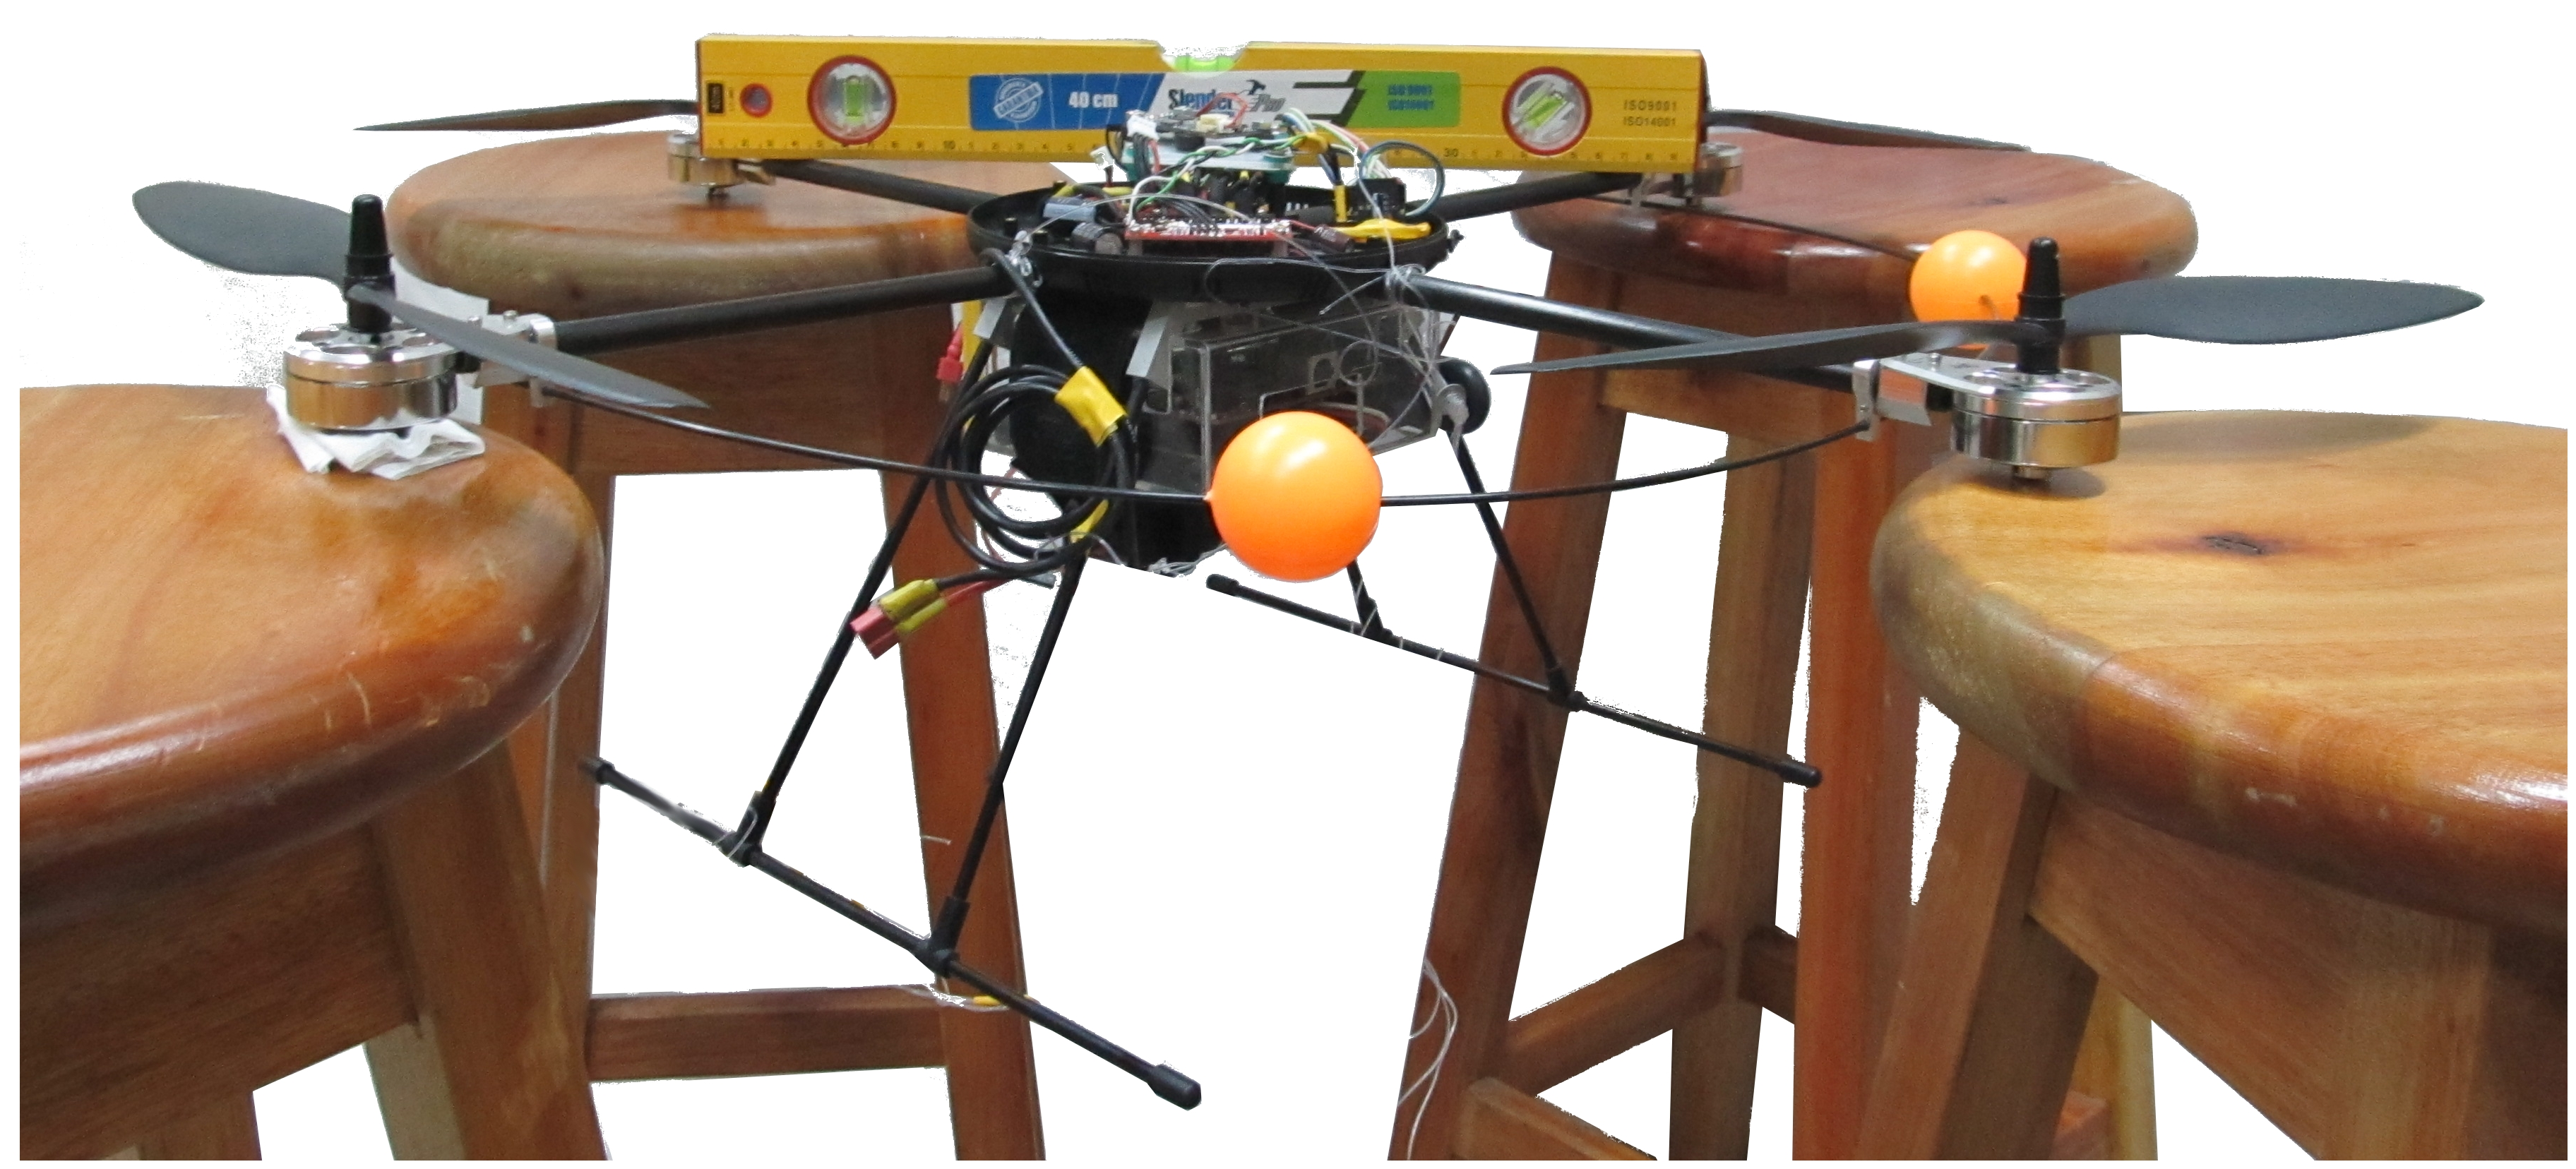
\includegraphics[width=0.5\textwidth]{./pics_montaje/horizontalidad.jpg}
	\end{center}
	\caption{Calibraci\'on de la vertical}
	\vspace{-10pt}
	\label{fig:horizontalidad}
\end{wrapfigure}

Otro aspecto fundamental para que las medidas de la IMU reflejen la realidad es la necesidad de ubicarla perfectamente horizontal. Para ello se utiliza el sistema mostrado en la figura \ref{fig:horizontalidad}, que aunque bastante precario, es efectivo. La idea es apoyar al cuadricóptero en los motores, simulando la fuerza que realizan en vuelo para compensar la fuerza del peso y lograr horizontalizar el plano de los brazos mediante la utilización de un nivel. Luego, ajustando o desajustando los tornillos se ubica la IMU de manera de obtener ángulos \emph{Roll} y \emph{Pitch} iguales a $0$.

\section{GPS}

\begin{wrapfigure}{r}{0.4\textwidth}
	\begin{center}
	\vspace{-45pt}
		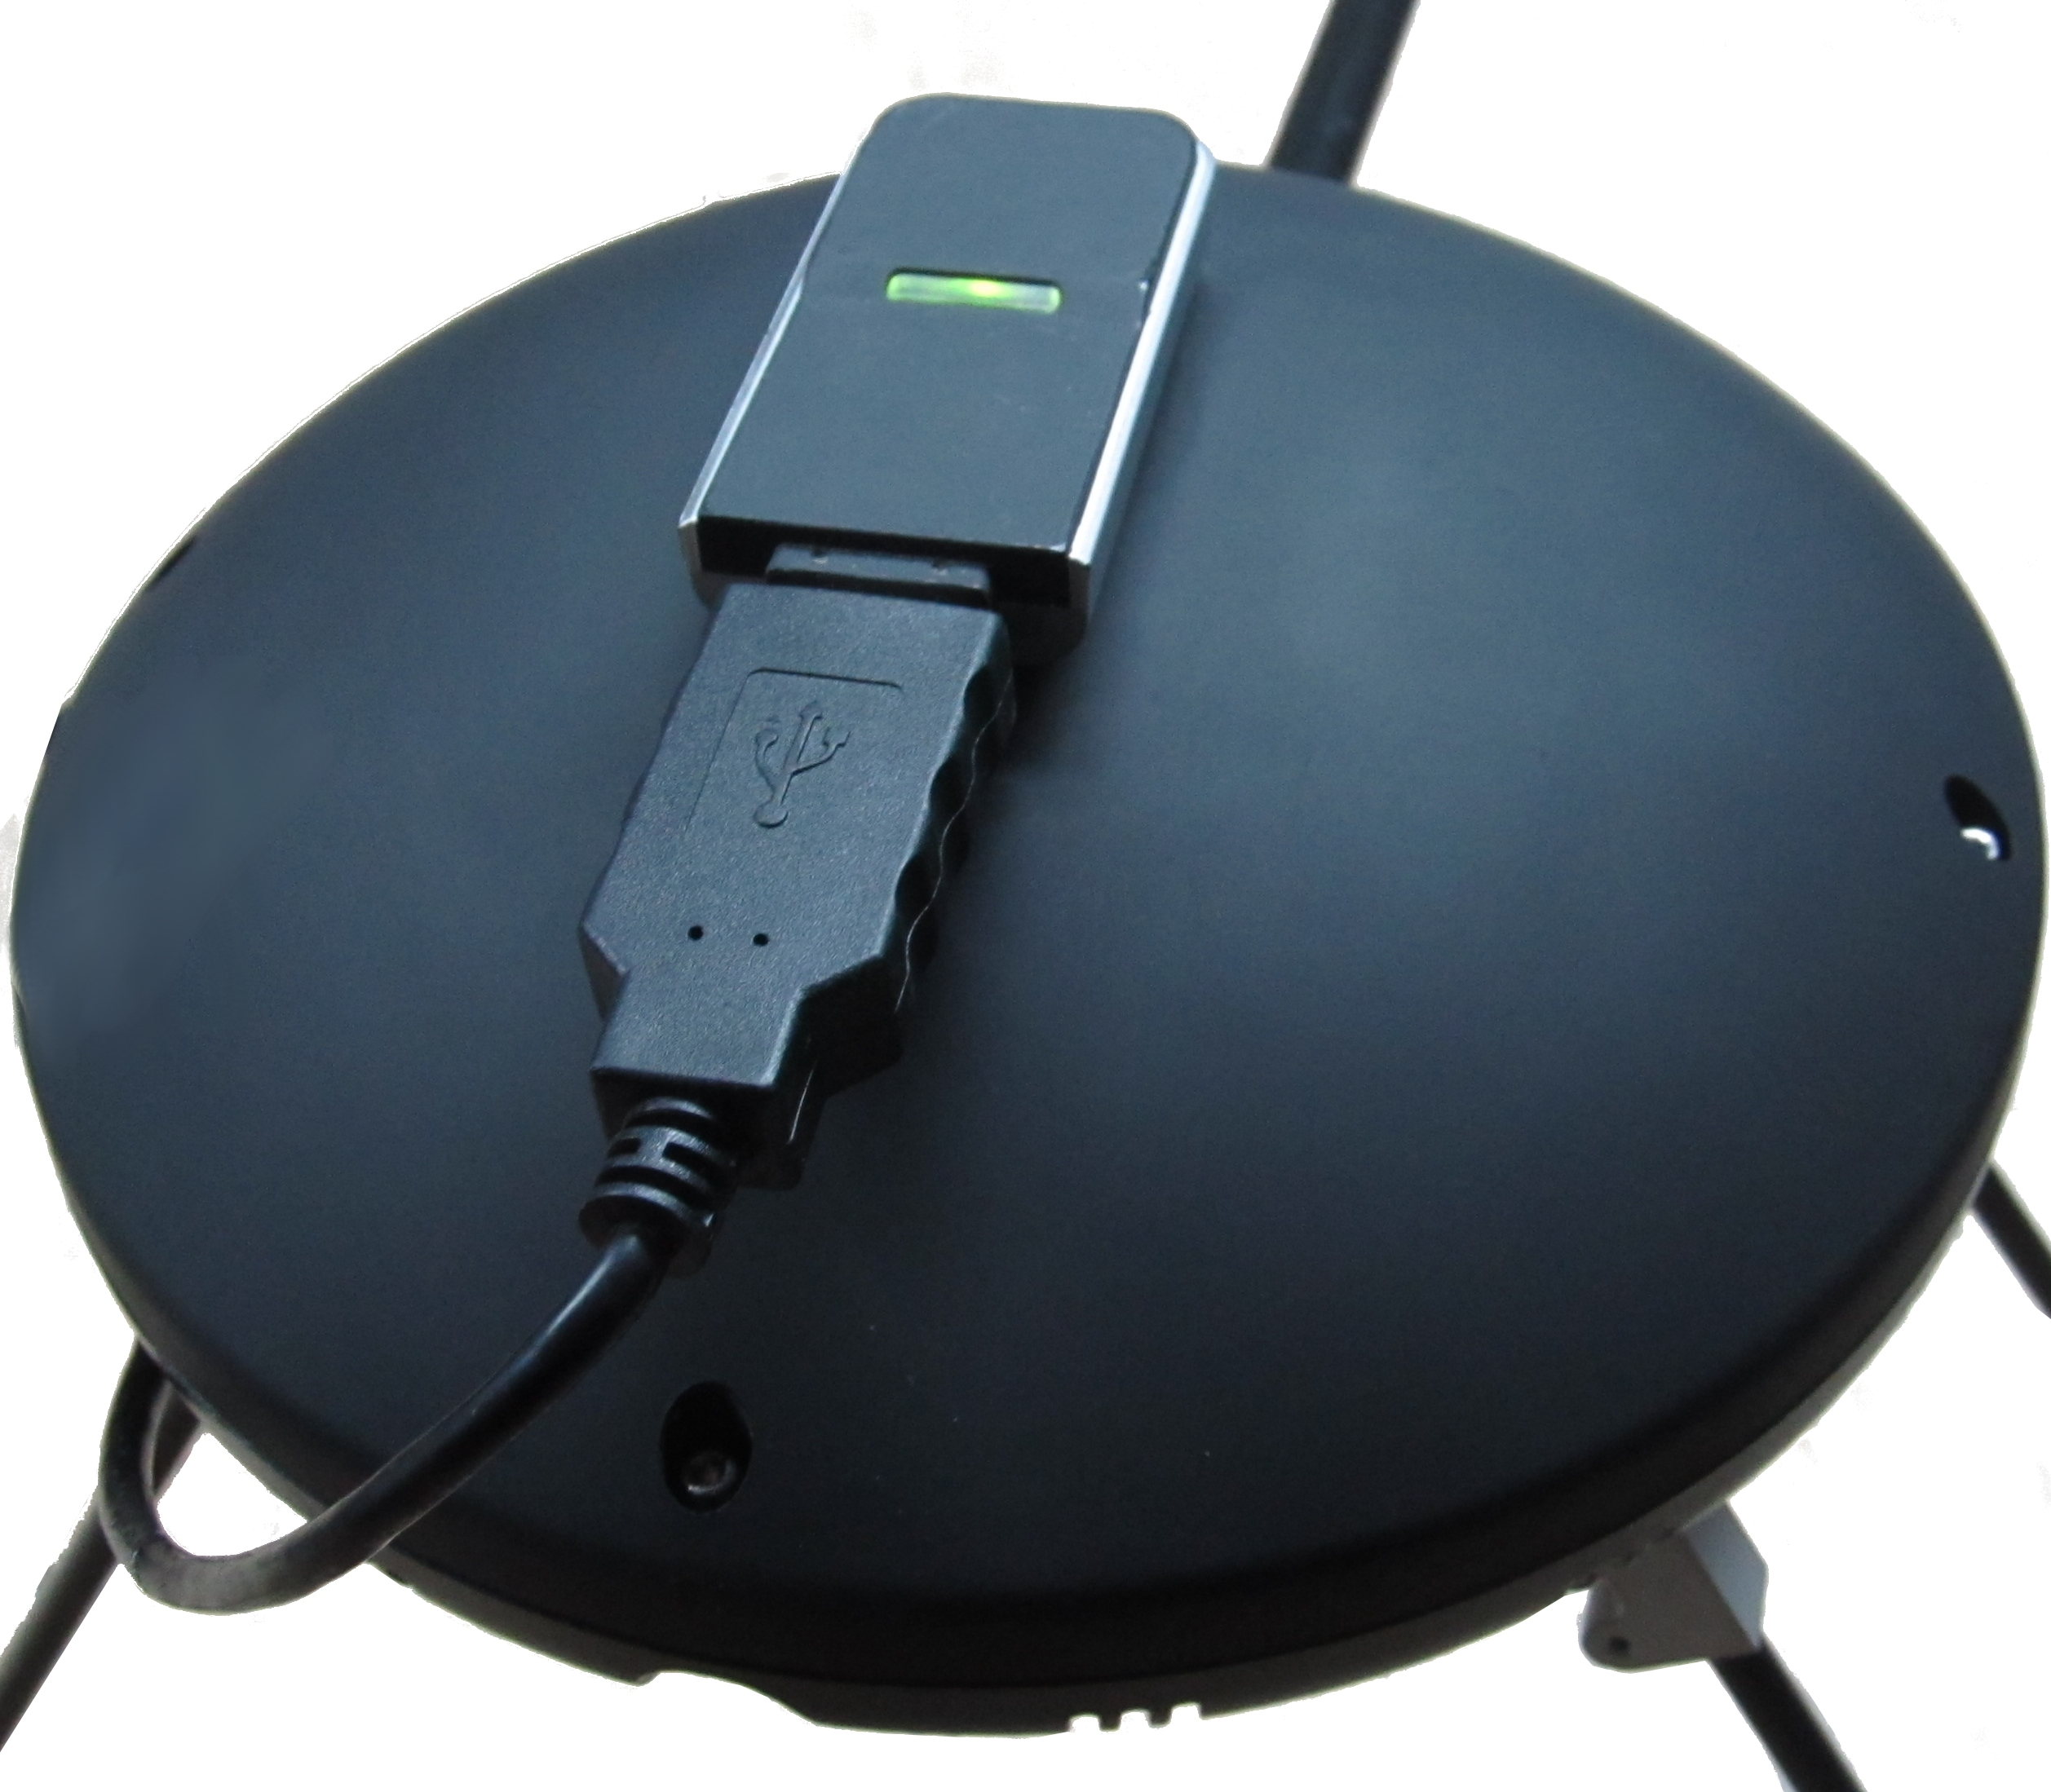
\includegraphics[width=0.3\textwidth]{./pics_montaje/gps.jpg}
	\end{center}
	\caption{Montaje del GPS}
	\vspace{-10pt}
	\label{fig:motaje_gps}
\end{wrapfigure}

El montaje del GPS se realiza de forma que tenga la mayor visibilidad de satélites posible. Como se mencionó en el capítulo \ref{chap-gps}, los rebotes en diferentes superficies provocan un deterioro considerable en la señal. Por estas razones se elige ubicarlo en la parte superior de la plataforma, como se muestra en la figura \ref{fig:montaje_gps}.

\vspace{25pt}

\section{Conversor lógico}

\begin{wrapfigure}{r}{0.5\textwidth}
	\begin{center}
	\vspace{-40pt}
		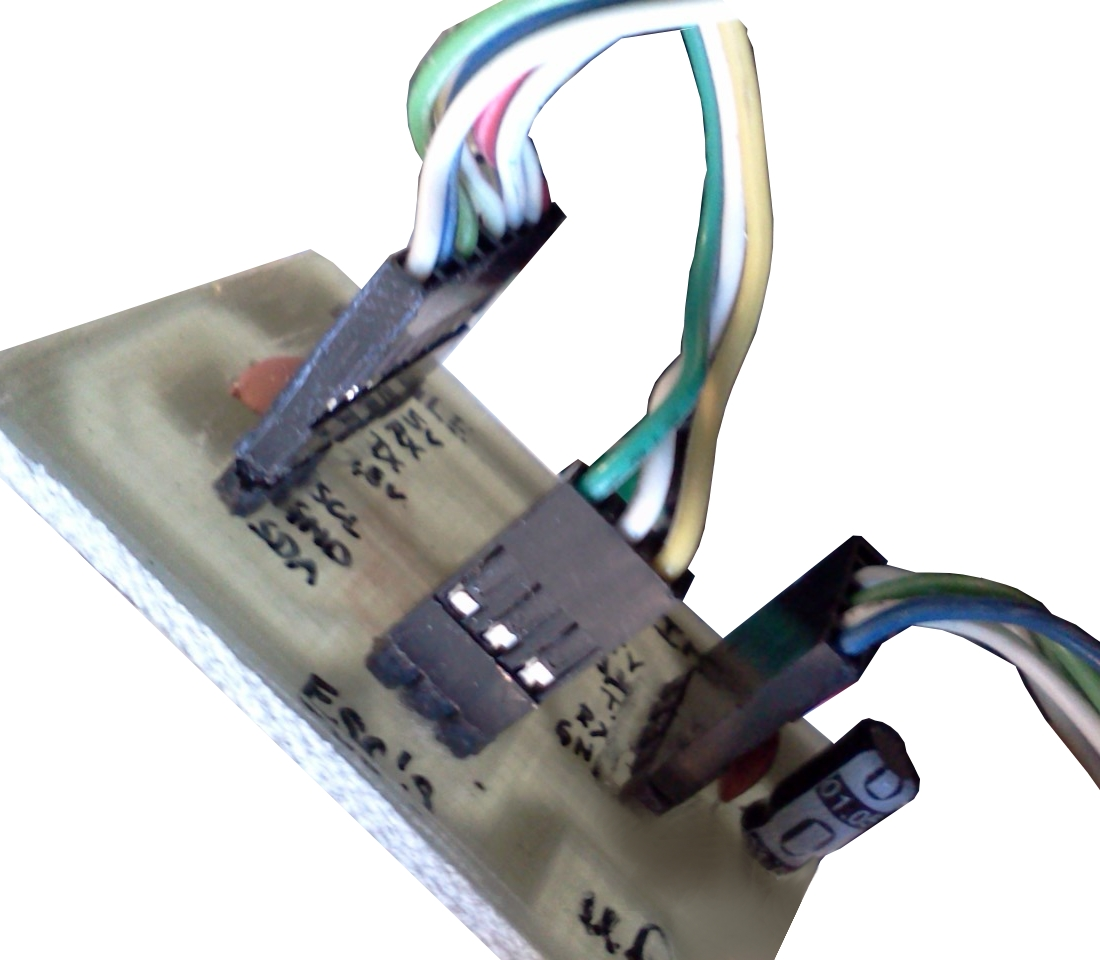
\includegraphics[width=0.35\textwidth]{./pics_montaje/cl.jpg}
	\end{center}
	\caption{Placa de conversores lógicos}
	\label{fig:cl}
\end{wrapfigure}

Como ya fue mencionado fue necesario la impresión de un circuito que convirtiera los voltajes entre las diferentes placas que componen el sistema. El mismo fue ubicado sobre 4 tuercas solidarias a la carrocería que se encontraban sin utilizar. La placa (mostrada en la figura \ref{fig:cl}), fue diseñada con el tamaño justo para atornillarse allí.

\end{document}